\subsection{Algorithm}

The algorithm is based on two main groups that are a list of \textit{basic functions} and list of \textit{binary operators} to combine them. This two lists are showed in table \ref{tab:BasicGroups}.
\begin{table}[h!]
	\centering
	\begin{tabular}{c|ccccccccc}
		\textbf{Basic functions} & \( 1 \) & \( \exp(x) \) & \( \sin(x) \) & \( x^2 \) & \( \tan(x) \) & \( \log(x) \) & \( |x| \) & \( a \) & \( x \) \\
		\hline
		\textbf{Basic operators} & \(a+b \) & \(a-b \) & \(a \cdot b \) & \(a \div b \) & \( a^b \) & & & &
	\end{tabular}
	\caption{Basic functions and binary operators.}
	\label{tab:BasicGroups}
\end{table}

The basic idea is to choose basic functions and combine them with some operators. But this could lead infinite possibilities, for this reason it was necessary to do some design choices.

\clearpage

\textbf{Rappresentation}

The functions are represented as \textit{Computational Graphs}. In figure \ref{fig:ComputationalGraph} is given an example of such representation, that refers to \Fig~\ref{fig:GeneralIdea}.
\begin{figure}[h!]
	\centering
	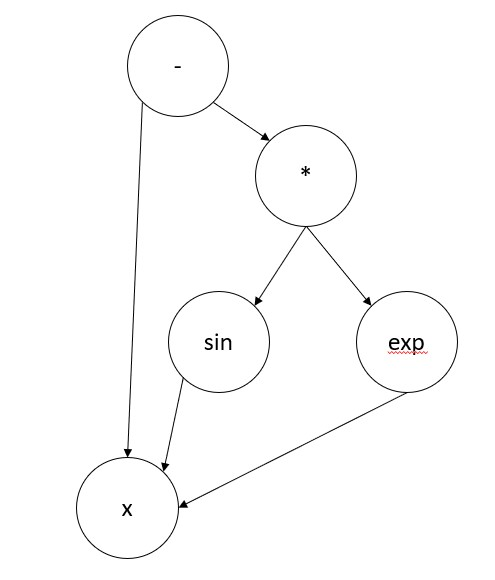
\includegraphics[width=0.2\linewidth]{./ImageFiles/Data Generation/ComputationalGraph}
	\caption{Computational graph example.}
	\label{fig:ComputationalGraph}
\end{figure} 

\textbf{Semplifications}

The first semplification is referred to the maximum number of children at each node that is two. Then the result is a binary graph. This does not limit the possible functions that can be generated.

The second semplification is the graph depth, that is kept less or equal than three. The depth is directly proportional to the function's complexity. Here are some examples for different complexity levels.

\begin{tabular}{c|c | c}
	Complexity level 1 & Complexity level 2 & Complexity level 3\\
	\hline
	$f(x) = sin(x) + x$ & $f(x) = tan(sin(x) + x)$ & $f(x) = tan(sin(x)+x) x^2$\\
	$f(x) = log(sin(x))$ & $f(x) = log(sin(x) x^2)$ & $f(x) = \frac{log(asin(x))}{x}$\\
	$f(x) = \frac{e^x}{x^2}$ & $f(x) = |\frac{e^x}{sin(x)}|$ & $f(x) = |\frac{e^x}{x} - \frac{a}{x}|$
\end{tabular}

\textbf{Generation}

The generation is made with different level of complexity to guarantee a fair distribution in the dataset. More precisely, 10\% is depth 1, 30\% depth 2 and 60\% depth 3. The precentage is proportional to the number of possible resulting functions.

Two datasets are generated, a reduced one with 2000 samples to do preliminary training and a larger one with 50000 samples.

\textbf{Adjustments}

Some more adjustments were made to the algorithm in order to get better datasets. The first problem was the huge presence of constant functions, e.g. a function like "$f(x) = sin(x) - sin(x)"$ is just a 0. Therefore, this kind of situations are managed.

Another problem was given by equivalent representations, e.g. "$f(x) = x + x$" and "$f(x) = 2x$" are the same functions but with different representation and this could lead to confusion in the model. This is not deleted at all but strongly mitigated.